\documentclass[12pt,leqno,twoside]{mwart}
\usepackage[polish]{babel}
\usepackage[utf8]{inputenc}
\usepackage[T1]{fontenc}
\usepackage{a4wide}
\usepackage[titles]{tocloft}
\usepackage{url}
\usepackage{graphicx}

\widowpenalty=10000
\clubpenalty=10000
\raggedbottom

%---------------------------------------------------------------------------------
%paginy!
\usepackage{fancyhdr}
\pagestyle{fancy}
\fancyhead{}
\renewcommand{\sectionmark}[1]{\markright{\thesection.\ #1. }}
\renewcommand{\sectionmark}[1]{\markright{\thesection.\ #1}}
\fancyhead[LE]{WiDz -- Wirtualny Dziennik. Architektura oprogramowania}
\fancyhead[RO]{\rightmark}
\fancyfoot{} % clear all footer fields
\fancyfoot[LE,RO]{}
\fancyfoot[CE]{\thepage}
\fancyfoot[CO]{\thepage}
\addtolength{\headheight}{1.5pt} % pionowy odstep na kreske
\renewcommand{\headrulewidth}{0.4pt}
\renewcommand{\footrulewidth}{0.0pt}
%--------------------------------------------------------------------------------

%\makeatletter
%\renewcommand{\@biblabel}[1]{\quad #1.}
%\makeatother

\renewcommand{\figurename}{Rys.}
\renewcommand{\labelitemi}{-}

%\makeatletter
%\renewcommand{\@pnumwidth}{1.75em}
%\renewcommand{\@tocrmarg}{2.75em}
%\makeatother

%\setlength{\cftbeforechapskip}{2ex}
%\setlength{\cftbeforesecskip}{0.5ex}

\begin{document}

\begin{titlepage}
\begin{center}
Instytut Informatyki Uniwersytetu Wrocławskiego \\
Studencka Pracownia Inżynierii Oprogramowania, G4 \\
\vspace{4cm}
\Large Michał Kopacz, Mateusz Nahalewicz, Karol Bajko \\
\vspace{0.5cm}
\huge Dokumentacja projektu \mbox{\textbf{WiDz -- Wirtualny Dziennik}} \\ \Large Architektura oprogramowania\\
\vspace{1cm}
\normalsize Wersja 1.2
\vfill
\normalsize Wrocław 2009
\end{center}
\end{titlepage}

\newpage
\vfill
\renewcommand*{\tablename}{Tabela}
\begin{table}
	\centering
	\caption{Historia zmian w~dokumencie}
		\begin{tabular}{|r|c|c|p{5,5cm}|l|}
		\hline
		Lp. 	& Data       & Nr wersji 	& Autor           		& Zmiana \\ \hline
		1.   	& 2009-12-15 & 1.0       	& \mbox{Karol Bajko} & Utworzenie dokumentu \\ \hline
		2.   	& 2010-01-10 & 1.1       	& \mbox{Karol Bajko} & Korekta \\ \hline
		3.   	& 2010-01-24 & 1.2       	& \mbox{Karol Bajko} & Korekta \\ \hline
		\end{tabular}
\end{table}

\tableofcontents
\newpage

\section{Wstęp}
% TODO: naprawić powtarzające się słowo 'architektura'
\noindent Niniejszy dokument ma na celu przedstawienie czytelnikowi architektury programu WiDz. Prezentuje jej kluczowe składniki, a także skupia się na analizie architektury z~kilku perspektyw -- logicznej, implementacyjnej, wdrożeniowej i procesowej. Wszystko po to, aby ułatwić potencjalnemu klientowi zrozumienie architektury programu WiDz.\\
\indent Opisana poniżej architektura może ulec zmianie w~fazie implementacji, lecz ogólny schemat programu nie powinien zostać naruszony.

\section{Elementy architektury WiDz}
\subsection{Serwer programu WiDz}
\noindent Serwer programu WiDz jest podstawowym składnikiem architektury, gdyż na nim zostanie uruchomiony program WiDz. Posiada on zainstalowany system operacyjny Linux i udostępnia interpreter języka Ruby, menadżera pakietów RubyGems do zarządzania bibliotekami koniecznymi do uruchomienia programu, oprogramowanie serwerowe \hbox{HTTP Apache} z~modułem Passenger, niezbędne do współpracy z~programem WiDz zbudowanym w~Ruby on Rails, bibliotekę kryptograficzną OpenSSL oraz SZBD MySQL.\\
\indent Serwer programu WiDz jest odpowiedzialny za umożliwienie stałego dostępu do programu WiDz każdemu użytkownikowi, bez względu na porę dnia. Odpowiada również za okresowe tworzenie kopii bezpieczeństwa danych znajdujących się w~bazie danych. 

\subsection{Baza danych}
\noindent Baza danych -- inaczej: system zarządzania bazą danych, SZBD -- przechowuje wszystkie dane związane z~oferowanymi usługami programu WiDz. Zawiera wszystkie dane dotyczące nauczycieli oraz uczniów i opiekunów. Baza danych przechowuje m.in. dane o postępach uczniów w nauce, o dokonanych opłatach, bieżącym planie zajęć w szkole oraz archiwizuje wszelkie wiadomości przesyłane pomiędzy użytkownikami WiDz.\\
\indent Baza danych  MySQL jest umieszczona na serwerze. Korzystać z~niej może wyłącznie program WiDz, który ma bezpośredni dostęp do danych w~niej umieszczonych. Komunikacja między programem a SZBD MySQL opiera się na języku zapytań SQL.

\subsection{Pliki źródłowe}
\noindent Kod źródłowy WiDz-a został napisany w~języku Ruby z wykorzystaniem ramy projektowej Ruby on Rails. Język ten okazał się najlepszy do budowy programu, ponieważ umożliwia szybkie i łatwe tworzenie rozbudowanych projektów, a ponadto większe skupienie na samych funkcjach programu WiDz. Konieczność niskopoziomowego kodowania jest w nim sprowadzona do minimum, gdyż Ruby on Rails ma mnóstwo gotowych do użycia, domyślnych konwencji i~bibliotek\footnote{Zasada konwencja ponad konfigurację (ang. \textit{convention over configuration}), zob. \tt{http://software}\rm{-} \tt{engineering.vazexqi.com/files/pattern.html}.}. Sam program został zbudowany z użyciem wzorca projektowego MVC\footnote{Model-widok-sterownik (ang.~\textit{Model-view-controller}), więcej informacji na temat MVC w~Ruby on Rails w~\cite{SP}.}:
\begin{itemize}
\item warstwa modelu odpowiedzialna za komunikację z~bazą danych i~przetwarzanie danych,
\item warstwa widoku odpowiedzialna za prezentowanie wyników działania programu na ekranie monitora,
\item warstwa sterownika odpowiedzialna za przechwytywanie żądań użytkownika i~na ich podstawie generowanie odpowiedzi, z pomocą dwóch powyższych warstw.
\end{itemize}

\subsection{Interfejs użytkownika}
\noindent Interfejs użytkownika to element bardzo istotny w~całym projekcie. Sukces programu zależy w~dużej mierze od jego intuicyjności, przejrzystości i~łatwości obsługi. Do jego zbudowania zostały użyte języki HTML, CSS i JavaScript, które nie wymagają od użytkownika korzystającego z WiDz-a dodatkowych zabiegów instalacyjnych na komputerze roboczym. Do uruchomienia programu wystarczy przeglądarka internetowa.

\section{Perspektywy architektoniczne}
\subsection{Perspektywa logiczna}
\noindent Perspektywa logiczna koncentruje się na strukturze projektu, budowie i~zależnościach klas charakterze użycia zewnętrznych bibliotek rozszerzających podstawowe funkcje programu.% Bardzo precyzyjny opis tych elementów, na obecnym etapie zaawansowania projektu, nie jest w~pełni możliwy. Dokładniejsze informacje zostaną przedstawione w~etapie implementacji.\\

\indent W~tabeli \ref{kluczowe_klasy} znajdują się informacje o~kluczowych klasach WiDz-a i przyporządkowanych im operacjach. Każda klasa, zgodnie z~zasadami Ruby on Rails, reprezentuje samodzielny zasób, który można łączyć z~innym zasobem aby w ten sposób tworzyć rozbudowane obiekty koncepcyjne. Każdy taki zasób ma zdefiniowane wszystkie operacje, które można na nim wykonywać. Dostęp do poszczególnych funkcji jest nadawany z uwzględnieniem typu użytkownika w konfiguracji klas. Taki styl projektowania, który skupia się głównie na zasobach, nosi nazwę REST\footnote{\textit{Representational State Transfer}, zob. \tt{http://www.ics.uci.edu/~fielding/pubs/dissertation/}\rm{-} \tt{top.htm}.}. Dokładniejsze zależności między klasami zostały zaprezentowane w~rozdziale \ref{UML}.
% TODO: "za pomocą" czy "przy pomocy"?
% TODO: referencja do kluczowe_klasy
\begin{table}[h]
	\centering
	\caption{Kluczowe klasy WiDz-a i~ich metody}
		\rule{0pt}{3ex}
		\begin{tabular}{|l|p{12cm}|}
		\hline
		\textbf{Klasa} & \textbf{Funkcje} \\ \hline
		Uzytkownik & uwierzytelnianie \\ \hline
		Uczen & 
			\parbox[t]{12cm}{
			\raggedright
				przegladaj\_uczniow, dane\_ucznia, dodaj\_ucznia, usun\_ucznia
			}\\ \hline
		Ocena & 
			\parbox[t]{12cm}{
			\raggedright
				przegladaj\_oceny, dane\_oceny, dodaj\_ocene, modyfikuj\_ocene, usun\_ocene
			} \\ \hline
		Frekwencja &
			\parbox[t]{12cm}{
			\raggedright			
				przegladaj\_frekwencje, dodaj\_frekwencje, modyfikuj\_frekwencje, usun\_frekwencje, usprawiedliw\_nieobecnosc
			}\\ \hline
		Nauczyciel &
			\parbox[t]{12cm}{
			\raggedright			
				przegladaj\_nauczycieli, dane\_nauczyciela, dodaj\_nauczyciela, modyfikuj\_nauczyciela, usun\_nauczyciela
			} \\ \hline
		Wychowawca & wyslij\_wiadomosc\_uczniom \\ \hline
		Opiekun & przegladaj\_opiekunow, dane\_opiekuna \\ \hline
		Klasa & dane\_klasy, przedmioty, plan\_zajec, nauczyciele \\ \hline
		Przedmiot &
			\parbox[t]{12cm}{
			\raggedright			
				przegladaj\_przedmioty, dane\_przedmiotu, dodaj\_przedmiot, modyfikuj\_przedmiot, usun\_przedmiot 
			}\\ \hline
		PlanLekcji &
			\parbox[t]{12cm}{
			\raggedright			
				przegladaj\_plany\_lekcji, dodaj\_plan\_lekcji, modyfikuj\_plan\_lekcji 
			}\\ \hline
		Platnosci &
			\parbox[t]{12cm}{
			\raggedright			
				przegladaj\_platnosci, dodaj\_platnosc, modyfikuj\_platnosci, usun\_platnosc, oplac\_platnosc 
			}\\ \hline
		Komunikacja & wyslij\_wiadomosc, wyslij\_sms, historia\_wiadomosci \\ \hline
		OcenaZajec &
			\parbox[t]{12cm}{
			\raggedright			
				dodaj\_ankiete, modyfikuj\_ankiete, wypelnij\_ankiete, wyniki\_ankiety 
			}\\ \hline
		Raporty & generuj\_swiadectwa, statystyka\_frekwencji, statystyka\_ocen \\ \hline
		\end{tabular}
	\label{kluczowe_klasy}
\end{table}

\subsubsection{Diagram UML klas programu WiDz}\label{UML}
\noindent Diagram UML reprezentujący zależności między klasami WiDz-a pokazano na rysunku \ref{fig:uml}. Dla większej czytelności pominięto zależności klasy Dyrektor i~Administrator z~innymi klasami, które mają dostęp do wszystkich funkcji i~informacji w~programie WiDz.

\indent Ponieważ w~programie użyto stylu projektowego REST, upoważnienia do poszczególnych funkcji nadaje się według typu użytkownika, zgodnie z wymaganiami postawionymi w dokumencie \cite{WYM}. Na diagramie pokazano techniczne relacje między klasami, zgodnie z~koncepcją realizacji projektu w~Ruby on Rails, z pominięciem dokładniejszych relacji związanych z funkcjami konkretnych użytkowników.
\begin{figure}[ht]
\center
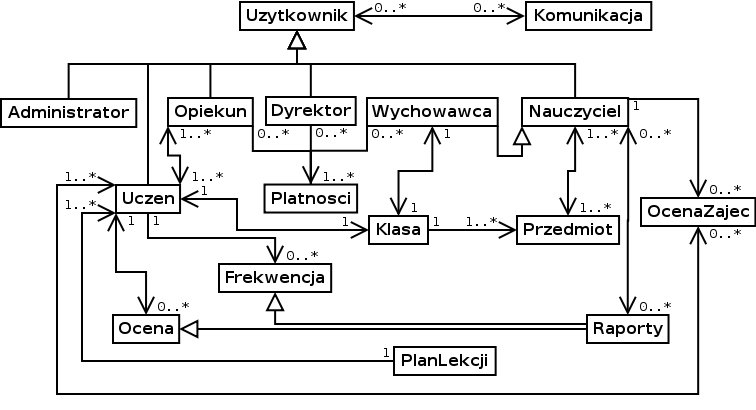
\includegraphics[width=16cm]{uml_klas.png}
\caption{Diagram UML reprezentujący zależności między klasami WiDz-a}
\label{fig:uml}
\end{figure}

\subsection{Perspektywa implementacyjna}
\noindent Perspektywa implementacyjna skupia się na ustaleniach sposobu kodowania oraz implementowania programu WiDz. Najważniejsze klasy i~zależności między nimi zostały już zaprezentowane w~poprzednim podrozdziale, zatem tutaj skupimy się głównie na samym środowisku, w~którym będzie tworzony program.

\indent Aby WiDz-a można było uznać za produkt najwyższej jakości, po każdym etapie implementacji nawet najmniejszego fragmentu kodu cały program powinien być testowany i~uruchamiany w~środowisku bardzo zbliżonym do tego, w~którym będzie eksploatowany po zakończeniu nad nim prac. W~tabeli \ref{elementy_architektury} dla przypomnienia zawarto istotne oprogramowanie, biblioteki oraz języki programowania użyte w~programie WiDz.

\indent Konfiguracja poszczególnych komponentów architektury została tak dopasowana do programu WiDz, by końcowy efekt był zgodny z~wymaganiami postawionymi w~dokumencie~\cite{WYM}. Struktura samej bazy danych odpowiada w~dużej mierze koncepcji klas, które zaprezentowano w~poprzednim podrozdziale.
\begin{table}[h]
	\centering
	\caption{Elementy architektury programu WiDz}
		\begin{tabular}{|l|p{10cm}|}
		\hline
		\textbf{Element architektury} & \textbf{Oprogramowanie, języki programowania} \\ \hline
		Serwer & HTTP Apache + moduł Passenger, rama Ruby on Rails, menadżer pakietów RubyGems \\ \hline
		Baza danych & SZBD MySQL na serwerze \\ \hline
		Pliki źródłowe & język Ruby, rama Ruby on Rails \\ \hline
		Interfejs użytkownika & witryna internetowa, języki HTML, CSS, JavaScript \\ \hline
		\end{tabular}
	\label{elementy_architektury}
\end{table}

\subsection{Perspektywa procesowa}
\noindent Poważnym problemem z~jakim może spotkać się w WiDz-u, jest jednoczesna obsługa nawet kilkuset użytkowników, którzy w~tym samym czasie będą korzystać z~programu. Wymagane więc jest, aby przepustowość łącza internetowego z serwerem była wystarczająca do jednoczesnego przesyłania dużej ilości danych. Minimalne wymagania sprzętowe serwera zostały przedstawione w dokumencie \cite{WYM}.

\subsection{Perspektywa wdrożeniowa}
\noindent Aby wdrożyć program WiDz, należy wykonać następujące czynności:
\begin{enumerate}
	\item Zainstalować i~skonfigurować na serwerze oprogramowanie serwerowe \hbox{HTTP Apache} wraz z modułem Passenger, interpreterem języka Ruby, menadżerem RubyGems, ramą projektową Ruby on Rails oraz podstawowymi bibliotekami\footnote{Instalowane za pomocą menadżera RubyGems, są to moduły: dbi, erector, god, json, mysql, net-ssh, rails, rake i rspec.} do użytku w~środowisku Ruby on Rails.
	\item Zainstalować i skonfigurować na serwerze SZBD MySQL.
	\item Skopiować pliki źródłowe WiDz-a na serwer.
	\item Zintegrować program WiDz z~SZBD MySQL i~oprogramowaniem serwerowym.
	\item Zainstalować i~skonfigurować program GOD\footnote{GOD - Process Monitoring Framework in Ruby -- program monitorujący uruchomione procesy na serwerze, dba o ich ciągłą obecność w~systemie.}.
	\item Uruchomić proces dbający o codzienne składowanie bazy danych.
\end{enumerate}

\section{Architektura a cechy projektu WiDz}
\subsection{Efektywność}
\noindent Wykorzystując pamięć podręczną po stronie użytkownika do składowania tymczasowych danych, odciążamy serwer od nadmiaru zadań, przerzucając ich część na użytkownika.
 
\subsection{Stabilność}
\noindent Bardzo rozbudowana biblioteka do testowania RSpec\footnote{Biblioteka BDD (ang. BDD --- \textit{Behavior-Driven Development}) dla aplikacji języka Ruby; umożliwia pisanie testów jednostkowych, opisujących konkretne obiekty oraz testów w~postaci scenariuszy opisujących zadania, które powinna wykonać aplikacja.} pomaga tworzyć testy dokładnie odpowiadające specyfikacji projektu, przez co wyłapywanie błędów i~ich naprawa odbywa się bardzo szybko. Rozwój użytych technologii w~WiDz-u sprawia, że program będzie zawsze zgodny z~najnowszymi wersjami systemów operacyjnych.

\subsection{Wygoda obsługi}
\noindent Przejrzysty, intuicyjny interfejs sprawia, że użytkownik nie ma problemów ze~swobodnym korzystaniem z~programu WiDz. Zastosowane języki HTML, CSS i JavaScript umożliwiają przyjazną interakcję z~użytkownikiem za pomocą przeglądarki internetowej. Bez względu na używany system operacyjny program zawsze wygląda tak samo.

\subsection{Możliwość rozwoju}
\noindent Zastosowany w~WiDz-u wzorzec projektowy MVC umożliwia rozszerzanie podstawowych funkcji programu o nowe działania. Mamy możliwość przekształcenia dziennika elektronicznego w~program, który obok pierwotnych funkcji, oferowałby funkcje przydatne w~zarządzaniu placówką szkolną, np. zautomatyzowany przepływ dokumentów pomiędzy osobami, szkołą a ministerstwem.

\indent Informatyzacja w~tej dziedzinie jest niezbędna, aby w~przyszłości proces kształcenia był efektywniejszy.

\section{Słownik}
%\begin{itemize}
%\item BDD
%\item CSS
%\item HTML
%\item JavaScript
%\item MVC
%\item środowisko developerskie
%\end{itemize}
\noindent Słownik terminów użytych w~dokumencie znajduje się w~\cite{SLO}.

\begin{thebibliography}{99}
\bibitem{SP} Edward Benson: {\it RAILS Sztuka Programowania}. Gliwice, Wydawnictwo HELION 2009.
\bibitem{WYM} Michał Kopacz, Mateusz Nahalewicz, Karol Bajko: {\it Dokumentacja projektu WiDz -- Wirtualny Dziennik. Specyfikacja wymagań}. Wrocław, SPIO IIUWr 2009.
\bibitem{SLO} Michał Kopacz, Mateusz Nahalewicz, Karol Bajko: {\it Dokumentacja projektu WiDz -- Wirtualny Dziennik. Słownik}. Wrocław, SPIO IIUWr 2009.
\end{thebibliography}

\end{document}
